\section{A Simple Motivating Example}
\label{sec:overview}

Consider a simple example of using \toolname: fixing broken list proofs after swapping the two list constructors (Figure~\ref{fig:listswap}).
This change is inspired by a similar change from a user study of proof engineers (Section~\ref{sec:search}).
Even such a simple change can cause trouble in proofs, like this proof from the Coq standard library:\footnote{We use induction instead of pattern matching.}

\begin{lstlisting}
Lemma rev_app_distr {A} :
  $\forall$ (x y : list A), rev (x ++ y) = rev y ++ rev x.(@\vspace{-0.04cm}@)
Proof.(@\vspace{-0.04cm}@)
  induction x as [| a l IHl].(@\vspace{-0.04cm}@)
  induction y as [| a l IHl].(@\vspace{-0.04cm}@)
  simpl. auto.(@\vspace{-0.04cm}@)
  simpl. rewrite app_nil_r; auto.(@\vspace{-0.04cm}@)
  intro y. simpl.(@\vspace{-0.04cm}@)
  rewrite (IHl y). rewrite app_assoc; trivial.(@\vspace{-0.04cm}@)
Qed.(@\vspace{-0.04cm}@)
\end{lstlisting}
This theorem says that appending two lists and reversing the result behaves the same way as appending
the reverse of the second list onto the reverse of the first list.
When we change the \lstinline{list} type, the proof no longer works.
%This theorem statement \lstinline{rev_app_distr} defined over the old version of \lstinline{list} is our \textit{old specification}.
%When we change the \lstinline{list} type, we get the \textit{new specification}.
%But the \textit{old proof} or tactic script no longer works with this new specification.
To repair this proof with \toolname, we just run this command:

\begin{figure}
%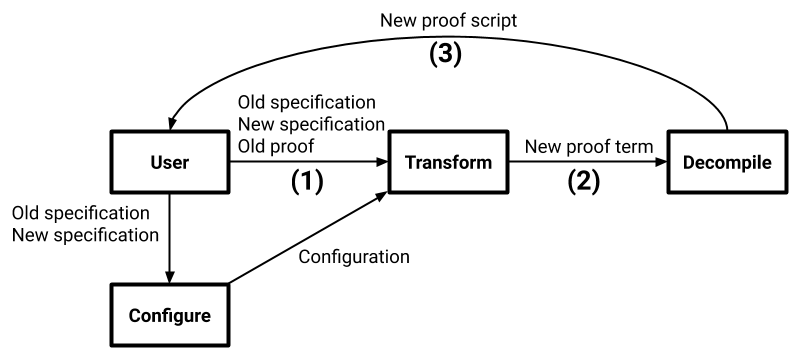
\includegraphics[width=\columnwidth]{workflowa.pdf}
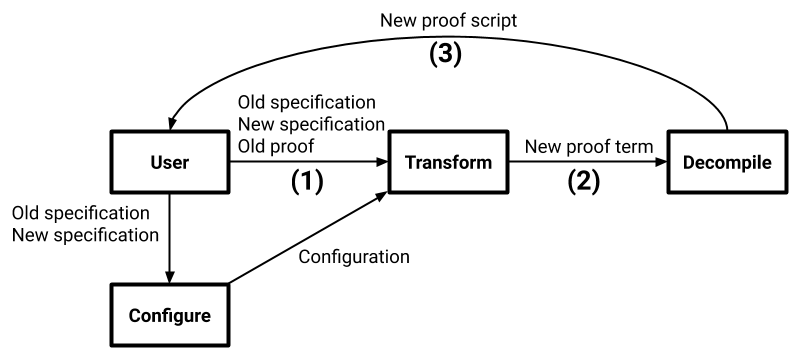
\includegraphics[width=\columnwidth]{workflowa.pdf}
\vspace{-0.5cm}
\caption{The workflow for \toolname.}
\label{fig:system}
\end{figure}

\begin{figure*}
\begin{minipage}{0.46\textwidth}
   \lstinputlisting[firstline=1, lastline=3]{listswap.tex}
\end{minipage}
\hfill
\begin{minipage}{0.46\textwidth}
   \lstinputlisting[firstline=5, lastline=7]{listswap.tex}
\end{minipage}
\vspace{-0.4cm}
\caption{The updated \lstinline{list} (right) is the old \lstinline{list} (left) with its two constructors swapped (\codediff{orange}).}
\label{fig:listswap}
\end{figure*}

\begin{figure*}
\codeauto{%
\begin{minipage}{0.48\textwidth}
\lstinputlisting[firstline=1, lastline=13]{equivproof.tex}
\end{minipage}
\hfill
\begin{minipage}{0.48\textwidth}
\lstinputlisting[firstline=15, lastline=28]{equivproof.tex}
\end{minipage}}
\vspace{-0.3cm}
\caption{Two functions between \lstinline{Old.list} and \lstinline{New.list} (top) that form an equivalence (bottom).}
\label{fig:equivalence}
\end{figure*}

\begin{lstlisting}
Repair Old.list New.list in rev_app_distr.(@\vspace{-0.04cm}@)
\end{lstlisting}
assuming the old and new list types from Figure~\ref{fig:listswap} are in modules \lstinline{Old} and \lstinline{New}.
This suggests an updated proof script that succeeds (in $\codeauto{light blue}$ to denote that it is produced automatically
by \toolname):

\begin{lstlisting}[backgroundcolor=\color{cyan!30}]
Proof.(@\vspace{-0.04cm}@)
  intros x. induction x as [a l IHl|]; intro y0.(@\vspace{-0.04cm}@)
  - simpl. rewrite (IHl y0). simpl.(@\vspace{-0.04cm}@)
    rewrite (app_assoc (rev y0) (rev l) (a::[])).(@\vspace{-0.04cm}@)
    auto.(@\vspace{-0.04cm}@)
  - induction y0 as [a l IHl|].(@\vspace{-0.04cm}@)
    + simpl. rewrite (app_nil_r (rev l) (a::[])).(@\vspace{-0.04cm}@)
      auto.(@\vspace{-0.04cm}@)
    + auto.(@\vspace{-0.04cm}@)
Qed.(@\vspace{-0.04cm}@)
\end{lstlisting}
where the dependencies (\lstinline{rev}, \lstinline{++}, \lstinline{app_assoc}, and \lstinline{app_nil_r}) have
also been updated automatically~\circled{1}. % Swap.v
If we would like, we can manually modify this to something that more closely matches the style of the original proof:

\begin{lstlisting}
Proof.(@\vspace{-0.04cm}@)
  induction x as [a l IHl|].(@\vspace{-0.04cm}@)
  intro y. simpl.(@\vspace{-0.04cm}@)
  rewrite (IHl y). rewrite app_assoc; trivial.(@\vspace{-0.04cm}@)
  induction y as [a l IHl|].(@\vspace{-0.04cm}@)
  simpl. rewrite app_nil_r; auto.(@\vspace{-0.04cm}@)
  simpl. auto.(@\vspace{-0.04cm}@)
Qed.(@\vspace{-0.04cm}@)
\end{lstlisting}
We can even repair the entire list module from the Coq standard library all at once by running the \lstinline{Repair module}
command~\circled{1}. % Swap.v
When we are done, we can get rid of \lstinline{Old.list}. % entirely.

The key to success here is taking advantage of Coq's structured proof term language:
Coq compiles every proof script to a proof term in a language called Gallina that is based on the calculus of inductive 
constructions---\toolname repairs that term.
\toolname then decompiles the repaired proof term back to a proof script that the proof engineer can maintain.
Here, \toolname transforms the proof term Coq compiles \lstinline{rev_app_distr} to,
and then decompiles that transformed proof term to the proof script in light blue.

In contrast, updating the poorly structured proof script directly would not be straightforward.
Even for the simple proof script above, grouping tactics by line, there are $6! = 720$ permutations of this proof script.
It is not clear which lines to swap since these tactics do not have a semantics beyond the searches their evaluation performs.
Furthermore, just swapping lines is not enough: even for such a simple change, we must also swap
arguments, so \lstinline{induction x as [| a l IHl]} becomes \lstinline{induction x as [a l IHl|]}.
%Handling even swapping constructors this way would require a search procedure that would not generalize to other changes.
\citet{robert2018} describes the challenges of repairing tactics in detail.

By instead transforming proof terms, \toolname is able to try just $1$ rather than $720$ candidates.
By decompiling the transformed proof term, \toolname is able to suggest a tactic script in the end.
As later sections show, this approach is much more general than just permuting constructors.



